\chapter{Methodology}
\label{chap:method}


% =================================================================
% 3.1 QCLand Overview
% =================================================================

\section{QCLand Overview}
\label{sec:method-overview}

Chapter 2 identified a gap between the transferable representations
offered by self-supervised vision foundation models, query-based
visual prediction, and the spatial precision required for fetal
biometry landmark localisation. QCLand addresses this gap by combining
landmark-query interaction, multi-depth spatial features, and
query-conditioned heatmap decoding within a pretrained vision
transformer.

The input ultrasound image is resized to $512 \times 512$ and passed
through a pretrained DINOv2 or DINOv3 backbone, which produces a
sequence of spatially grounded patch tokens. Two learned landmark
queries, one for each landmark channel, are inserted into the token
sequence partway through the backbone. During the remaining
transformer blocks, the queries interact with the patch tokens through
the backbone's own self-attention and form landmark-specific
representations. Features from multiple backbone depths are fused into
a shared spatial representation, while the final landmark-query
embeddings retain query-specific information. DeconvHeadV2 combines
these two inputs to produce a $64 \times 64$ heatmap for each
landmark, from which the corresponding coordinate is recovered.

Each fetal measurement is modelled independently: a separate QCLand
model is trained for each measurement, with two queries representing
its two landmarks.

\Cref{fig:qcland-architecture} illustrates the complete architecture.
The remainder of this chapter describes the landmark-query backbone,
the query-conditioned spatial decoder, multi-depth feature fusion,
the training objective, coordinate handling, and the training and
inference procedures.

\begin{figure}[!ht]
  \centering
  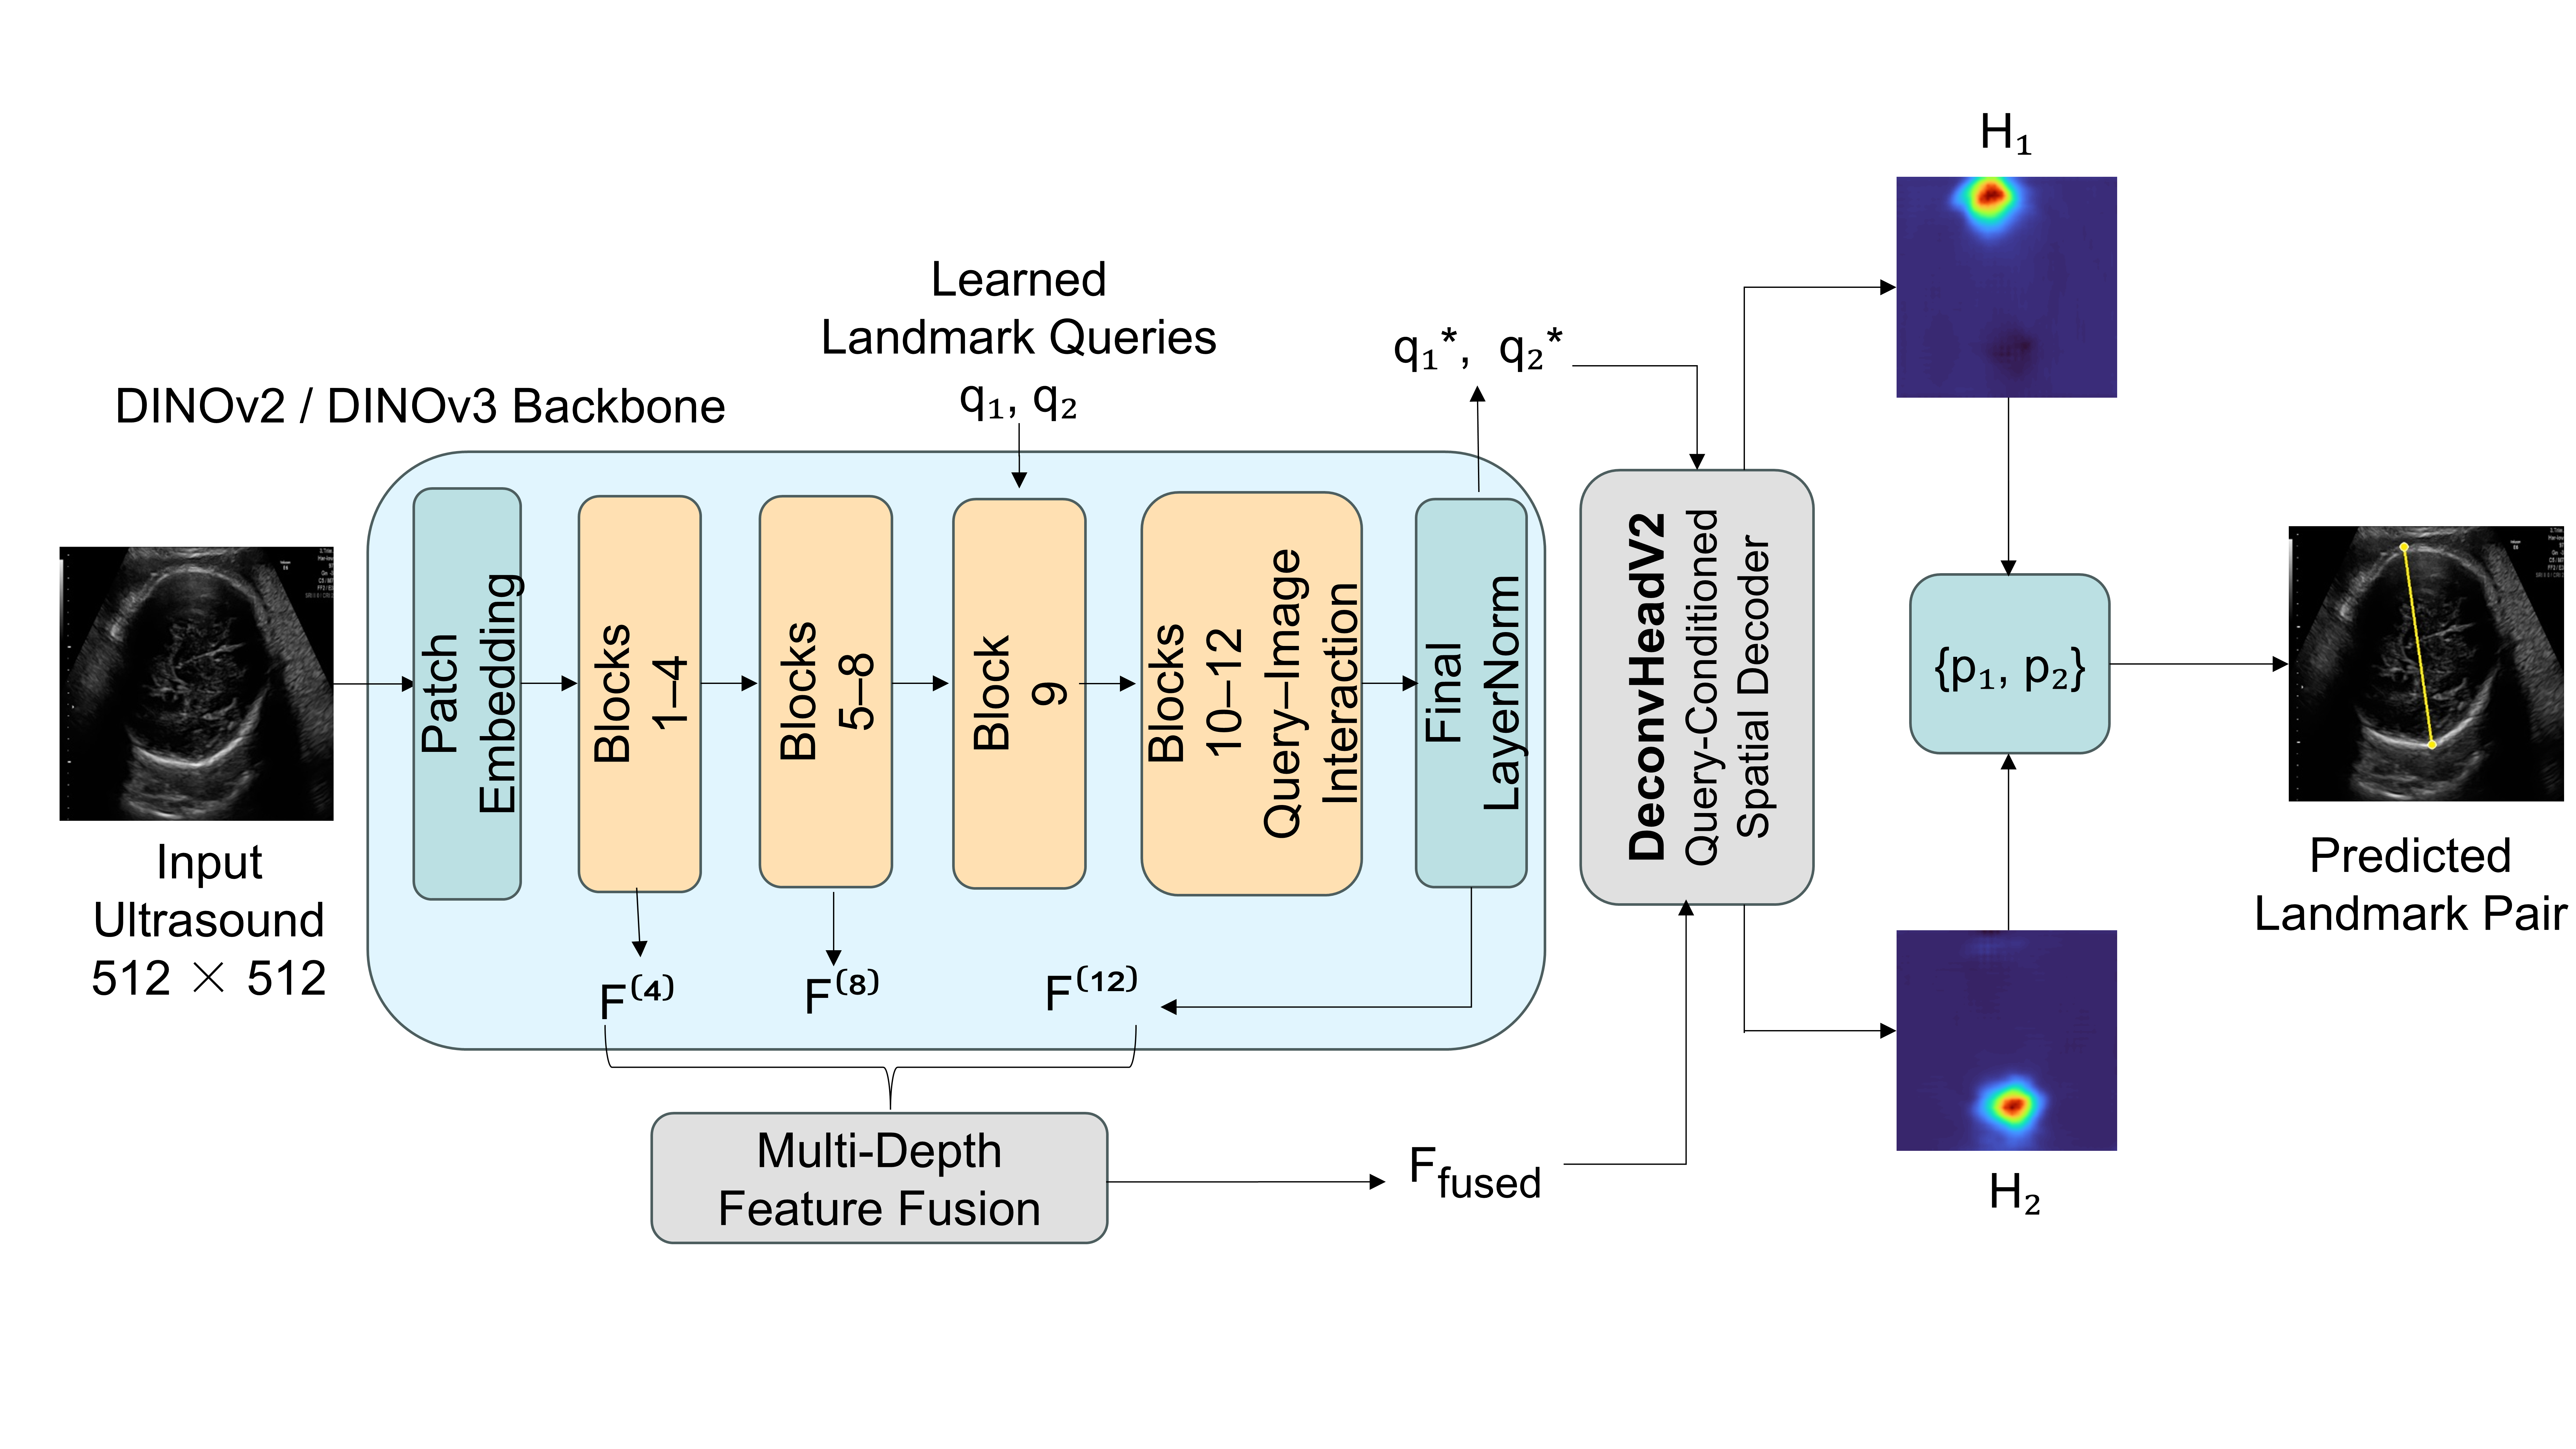
\includegraphics[width=\textwidth]
    {figures/qcland_overall_architecture.png}
  \caption[QCLand overall architecture]{Overall architecture of
    QCLand. A pretrained DINOv2 or DINOv3 backbone processes the
    input ultrasound image while two learned landmark queries
    interact with patch tokens through the final transformer blocks.
    Multi-depth patch features are fused into a shared spatial
    representation, while the final query embeddings provide
    landmark-specific conditioning. DeconvHeadV2 combines these two
    inputs to produce one heatmap for each landmark, from which the
    predicted landmark pair is recovered.}
  \label{fig:qcland-architecture}
\end{figure}


% =================================================================
% 3.2 Landmark Queries and Backbone Adaptation
% =================================================================

\section{Landmark Queries and Backbone Adaptation}
\label{sec:method-queries}

QCLand adapts a pretrained vision foundation model in two connected
ways: the backbone is fine-tuned to the fetal ultrasound domain,
while learned landmark queries are inserted into its final
transformer blocks to form landmark-specific representations. These
two components establish the representation used by the subsequent
spatial decoding stages.


\subsection{DINOv2 and DINOv3 Backbones}
\label{sec:method-backbone}

QCLand uses a pretrained vision transformer as its feature extractor.
Two backbone families are evaluated: DINOv2
\parencite{oquab2023dinov2} and DINOv3
\parencite{simeoni2025dinov3}. They share the same downstream
architecture and training framework; only the pretrained backbone
differs. The resulting variants are referred to as QCLand-DINOv2 and
QCLand-DINOv3 throughout this thesis.

Both backbones are initialised from pretrained weights and fine-tuned
jointly with the downstream QCLand components. Earlier transformer
blocks are adapted more conservatively through layer-wise
learning-rate decay, following established ViT fine-tuning practice
\parencite{bao2022beit}. For backbone block $i$ in an $L$-block
transformer,

\begin{equation}
  \label{eq:llrd}
  \mathrm{lr}_i
  =
  \mathrm{lr}_0
  \cdot
  \rho^{\,L-1-i},
\end{equation}

where $\mathrm{lr}_0 = 10^{-4}$ is the base learning rate,
$\rho = 0.8$, and $L=12$ for the backbones used here. The final block
therefore trains at the full base rate, while progressively earlier
blocks receive smaller learning rates. Non-backbone parameters,
including the landmark queries, DeconvHeadV2, and the fusion module,
are trained at the base rate. The backbone learning rate is held at
zero for the first 15 optimisation steps, allowing the newly
initialised downstream components to begin adapting before backbone
fine-tuning starts.

The DINOv2 configuration uses the ViT-S/14 register-token variant
\parencite{darcet2024registers}, with the patch-embedding kernel
resampled to $16 \times 16$ at load time. DINOv3 is natively
patch-16. Both variants therefore operate on the same
$32 \times 32$ patch-token grid for a $512 \times 512$ input,
although their positional encodings differ: DINOv2 uses learned
absolute position embeddings, whereas DINOv3 uses rotary position
embeddings.


\subsection{Landmark Queries}
\label{sec:method-landmark-queries}

Two learned query embeddings are initialised at random and inserted
into the token sequence starting $K$ blocks before the end of the
backbone, with $K=3$ in all experiments. The queries therefore
participate in blocks 10--12 together with the image and prefix
tokens. Through the backbone's own self-attention, they progressively
form landmark-specific representations by interacting directly with
the visual features.

No separate cross-attention or transformer decoder is required for
this interaction; the pretrained transformer blocks serve both as the
feature extractor and as the query--image interaction mechanism. This
query-in-encoder principle follows EoMT
\parencite{kerssies2025eomt}, while QCLand uses a fixed pair of
queries for landmark localisation.

At each of the $K$ query-interacting blocks, an auxiliary prediction
is produced using a lightweight dot-product readout
(\Cref{eq:bg-einsum}). The auxiliary predictions provide
deep-supervision loss terms during training and generate binary
attention masks that restrict each query's attention to currently
relevant image regions in the following block. Only the final
prediction, decoded through DeconvHeadV2 after the last transformer
block, is used to recover the reported landmark coordinates.


% =================================================================
% 3.3 Query-Conditioned Spatial Decoding
% =================================================================

\section{Query-Conditioned Spatial Decoding}
\label{sec:method-decoder}


\subsection{Why Spatial Decoding Is Needed}
\label{sec:method-decoder-motivation}

After the final transformer block, each landmark query contains a
representation relevant to its target landmark. Converting this
representation into a precise coordinate requires a spatial readout.
The auxiliary dot-product readout (\Cref{eq:bg-einsum}) forms each
output value independently at each spatial location, with no
subsequent local spatial mixing. Its ability to produce sharply
concentrated landmark responses is therefore not guaranteed by the
representation alone, motivating an explicit spatial decoding path
for the final prediction.


\subsection{DeconvHeadV2}
\label{sec:method-deconvheadv2}

DeconvHeadV2 is QCLand's principal architectural contribution. It
replaces the dot-product readout used for the auxiliary predictions
with a query-conditioned spatial decoding path for the final
prediction.

Before entering DeconvHeadV2, the fused spatial representation is
passed through a shared learned upsampling stage comprising two
ScaleBlocks. Each ScaleBlock doubles the spatial resolution using a
transposed convolution followed by local feature processing. Starting
from the $32 \times 32$ patch grid, the two blocks produce an
upsampled spatial representation

\[
F \in \mathbb{R}^{B \times 384 \times 128 \times 128}.
\]

DeconvHeadV2 receives this spatial representation together with the
final landmark-query embeddings. The spatial features are first
normalised using GroupNorm \parencite{wu2018groupnorm}. Each
landmark-query embedding is passed through a small MLP to predict
Feature-wise Linear Modulation (FiLM) parameters
\parencite{perez2018film}: a scale $\gamma_n$ and a shift $\beta_n$.
The normalised spatial feature map is then modulated independently for
each query:

\begin{equation}
  \label{eq:film-modulation}
  F'_n(x,y)
  =
  \gamma_n
  \odot
  \mathrm{GN}(F)(x,y)
  +
  \beta_n .
\end{equation}

The same spatial representation $F$ is therefore reused for both
landmark queries, while the query-specific FiLM parameters determine
how that representation is modulated for each landmark.

Each modulated feature map is subsequently passed through the same
shared convolutional decoder:

\begin{equation*}
  F'_n
  \xrightarrow{\;
    \mathrm{Conv}_{3\times3}
    \to
    \mathrm{ReLU}
    \to
    \mathrm{Conv}_{3\times3}
  \;}
  \widetilde{H}_n .
\end{equation*}

The first convolution reduces the channel dimension from 384 to 128,
and the second maps the 128-channel representation to a single
response map. The two landmark-query branches share these convolutional
weights; their outputs differ through the query-specific FiLM
modulation. The resulting $128 \times 128$ response map is finally
resized bilinearly to the target $64 \times 64$ landmark heatmap
$H_n$.

\Cref{fig:deconvheadv2-architecture} summarises this decoding pathway.

\begin{figure}[!ht]
  \centering
  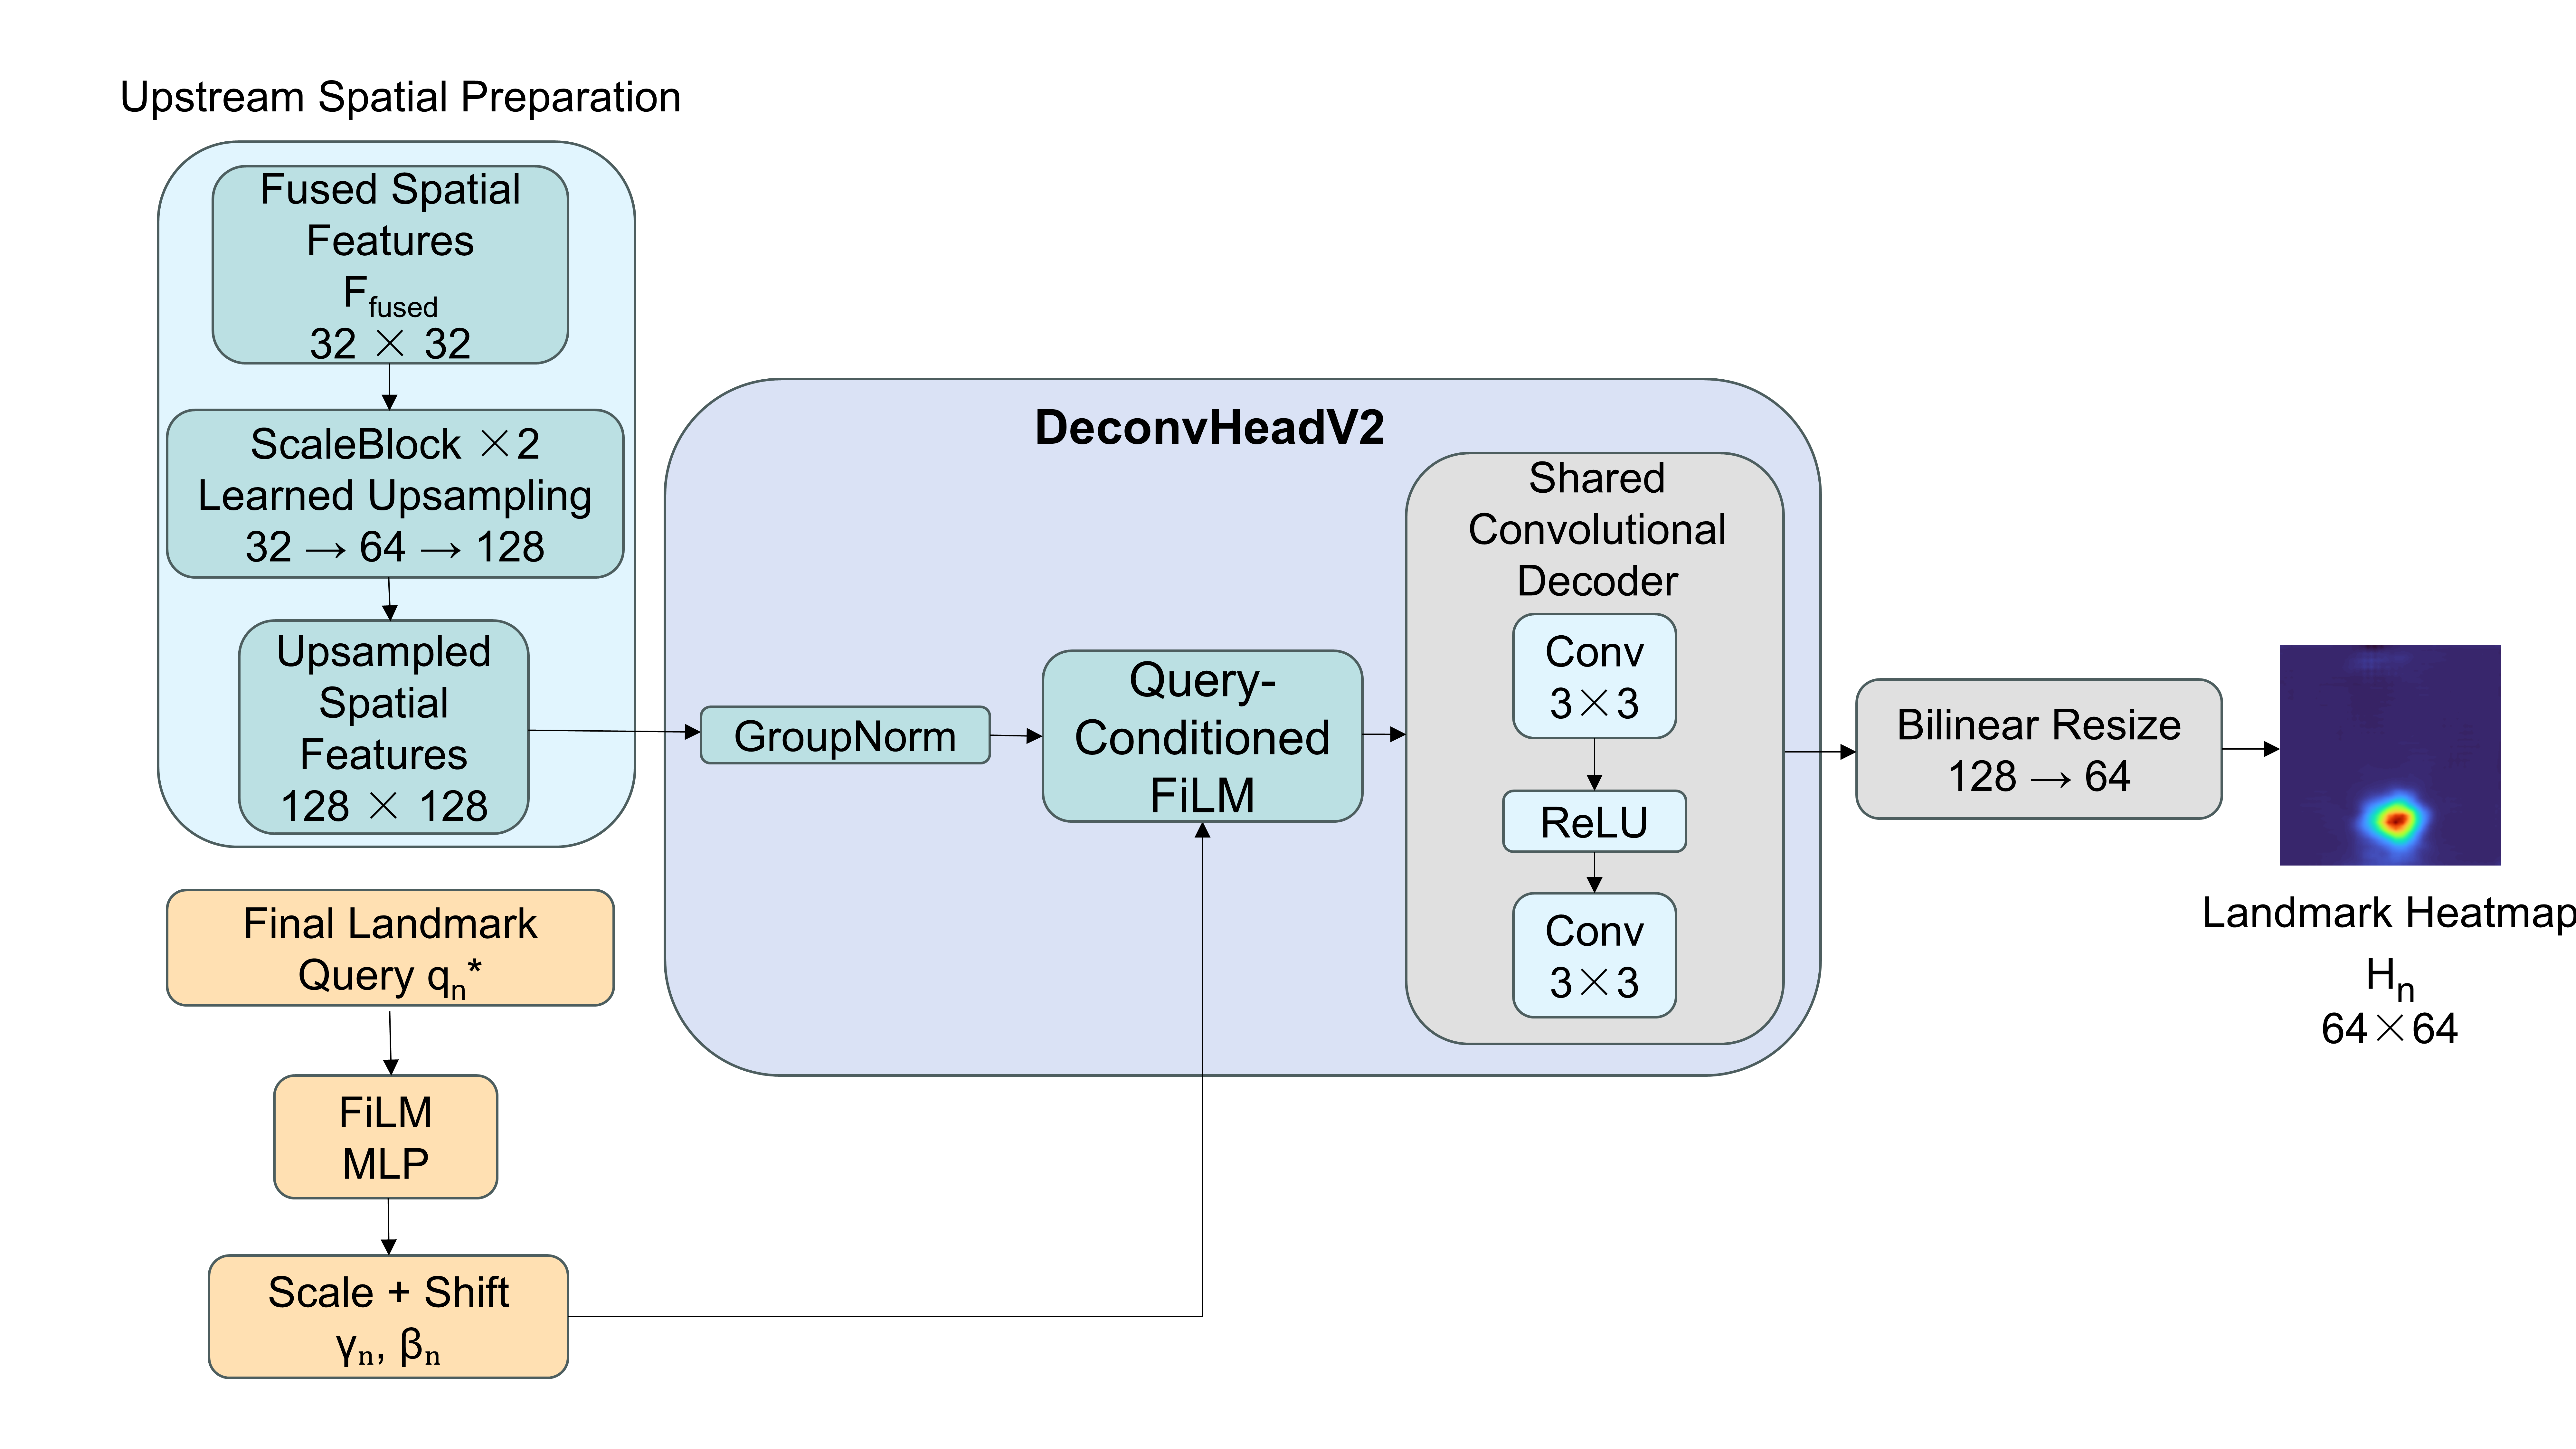
\includegraphics[width=\textwidth]
    {figures/deconvheadv2_decoding_pathway.png}
  \caption[DeconvHeadV2 decoding pathway]{DeconvHeadV2 decoding
    pathway. Fused multi-depth spatial features are first upsampled
    from $32\times32$ to $128\times128$. Inside DeconvHeadV2, the
    spatial representation is normalised and modulated by
    query-specific FiLM scale and shift parameters derived from each
    final landmark query. A convolutional decoder shared across
    landmark queries then produces a query-conditioned response map,
    which is bilinearly resized to the $64\times64$ landmark heatmap
    $H_n$.}
  \label{fig:deconvheadv2-architecture}
\end{figure}

The distinction from the auxiliary dot-product readout lies in the
spatial processing that follows query conditioning. Whereas the
dot-product formulation produces each spatial response independently,
DeconvHeadV2 applies shared convolutions over local neighbourhoods
after FiLM modulation, allowing the query-conditioned response to be
spatially refined. FiLM conditioning, GroupNorm, the shared
convolutions, and their initialisation form a single architectural
change relative to the dot-product readout; their effects are
therefore evaluated together rather than attributed to individual
subcomponents.


% =================================================================
% 3.4 Multi-Depth Feature Fusion
% =================================================================

\section{Multi-Depth Feature Fusion}
\label{sec:method-fusion}

Because a vision transformer's patch-token grid maintains the same
spatial resolution throughout the backbone, representations from
different depths remain spatially aligned while encoding different
stages of visual processing. QCLand exploits this alignment by fusing
spatial patch-token features from blocks 4, 8, and 12.

The shallower feature maps, $F^{(4)}$ and $F^{(8)}$, are captured
before the landmark queries are inserted into the token sequence.
They therefore represent image-only patch-token features at those
depths. The deepest feature map, $F^{(12)}$, is different. After the
queries are inserted before block 10, blocks 10--12 jointly process
the landmark queries, prefix tokens, and patch tokens through
self-attention. Following block 12, the backbone's final LayerNorm is
applied to the complete token sequence, after which the query and
prefix tokens are removed and the remaining patch tokens are reshaped
into a spatial feature map. Accordingly, $F^{(12)}$ denotes the
post-LayerNorm spatial patch-token features extracted after
query--image interaction through blocks 10--12.

QCLand therefore combines two pre-query representations,
$F^{(4)}$ and $F^{(8)}$, with the deepest query-interacted
representation, $F^{(12)}$. Blocks 4, 8, and 12 provide approximately
evenly spaced depths across the 12-block backbone; their selection was
not obtained through a search over alternative depth combinations.

Each feature map is independently normalised with GroupNorm. The three
normalised representations are concatenated along the channel
dimension and projected back to the backbone embedding dimension using
a $1 \times 1$ convolution. Because all three feature maps share the
same spatial grid, no top-down resizing pathway is required, unlike
the convolutional feature-pyramid architecture that motivated the
general multi-level fusion principle \parencite{lin2017fpn}.

The $1 \times 1$ projection is initialised such that only the deepest
feature level contributes at the start of training. The shallower
representations must therefore acquire useful fusion weights during
optimisation rather than perturbing the pretrained deepest
representation immediately.


% =================================================================
% 3.5 Landmark Targets and Training Objective
% =================================================================

\section{Landmark Targets and Training Objective}
\label{sec:method-objective}


\subsection{Heatmap Targets}
\label{sec:method-targets}

Following standard heatmap-based landmark supervision
\parencite{tompson2014joint,newell2016hourglass}, each landmark's
training target is a 2D Gaussian centred on the ground-truth
location, truncated to zero outside a square window of half-width
$\lfloor 3\sigma \rfloor$ pixels:

\begin{equation}
  \label{eq:gaussian-target}
  T_n(x,y) =
  \begin{cases}
    \exp\!\left(
      -\dfrac{
        (x-\mu_{x,n})^2 + (y-\mu_{y,n})^2
      }{2\sigma^2}
    \right),
    &
    |x-\mu_{x,n}|,\,
    |y-\mu_{y,n}|
    \le
    \lfloor 3\sigma \rfloor,
    \\[4pt]
    0,
    &
    \text{otherwise},
  \end{cases}
\end{equation}

where $(\mu_{x,n},\mu_{y,n})$ is the nearest heatmap pixel to the
continuous ground-truth coordinate and $\sigma=4.0$ for all fetal
experiments. The target is unnormalised with peak value 1.


\subsection{Hybrid Heatmap--Coordinate Loss}
\label{sec:method-losses}

The training objective combines a weighted heatmap term with a
coordinate-space term. The heatmap term reweights the per-pixel
squared error according to the target response:

\begin{equation}
  \label{eq:wmse}
  L_{\text{hm}}
  =
  \frac{1}{BNHW}
  \sum_{b,n,x,y}
  \bigl(1+\alpha T_{b,n}(x,y)\bigr)
  \bigl(
    \hat{H}_{b,n}(x,y)-T_{b,n}(x,y)
  \bigr)^2 .
\end{equation}

With $\alpha=5.0$, pixels at the target peak receive six times the
weight of background pixels. This foreground--background imbalance is
a known issue in landmark heatmap regression
\parencite{wang2019awing}: most locations in a $64\times64$ target
map are close to zero, so an unweighted objective can make globally
weak responses comparatively inexpensive.

A coordinate prediction is additionally extracted using a
differentiable spatial expectation (soft-argmax)
\parencite{sun2018integral}:

\begin{equation}
  \label{eq:soft-argmax}
  \hat{p}_n^{\text{soft}}
  =
  \sum_{x,y}
  (x,y)
  \cdot
  \frac{
    \exp(\tau\hat{H}_n(x,y))
  }{
    \sum_{x',y'}
    \exp(\tau\hat{H}_n(x',y'))
  },
\end{equation}

with temperature $\tau=10$. An L1 loss between this soft-decoded
coordinate and the continuous ground-truth coordinate provides a
direct spatial-precision signal:

\begin{equation}
  \label{eq:hybrid-loss}
  L
  =
  L_{\text{hm}}
  +
  \lambda_{\text{coord}}
  \cdot
  \frac{1}{2BN}
  \sum_{b,n}
  \left\lVert
    \hat{p}_{b,n}^{\text{soft}}
    -
    p_{b,n}
  \right\rVert_1,
  \qquad
  \lambda_{\text{coord}}=0.1 .
\end{equation}

The heatmap target is centred on a quantised pixel location, whereas
the coordinate term is supervised against the original continuous
coordinate. The two terms therefore provide complementary
supervision: the heatmap term shapes the spatial response, while the
coordinate term retains localisation information that heatmap
quantisation would otherwise discard.

The overall training loss is the equal-weighted average of $K+1$
per-layer terms: $K=3$ auxiliary dot-product losses and one
DeconvHeadV2 loss, each computed using the hybrid objective above.


% =================================================================
% 3.6 Coordinate Handling and Landmark Assignment
% =================================================================

\section{Coordinate Handling and Landmark Assignment}
\label{sec:method-coordinates}


\subsection{Landmark Assignment}
\label{sec:method-formulation}

The two landmarks defining each fetal measurement are treated as an
unordered pair for evaluation and do not carry persistent
query-specific anatomical identities in the training formulation.
During training, the pair is canonicalised from left to right by
$x$-coordinate in the current image coordinate system
\emph{after} any geometric augmentation has been applied. Query 0 is
assigned to the landmark with the smaller $x$-coordinate and query 1
to the landmark with the larger $x$-coordinate. The assignment is
recomputed for every sample and therefore does not encode a persistent
anatomical identity for either query.

For measurements whose two landmarks have little horizontal
separation, small geometric perturbations can reverse this ordering,
causing the same anatomical landmark to be assigned to different
queries across augmented views of an image. This behaviour follows
from the training-time canonicalisation rather than from an ambiguity
in the clinical measurement itself. Because the ordering convention
has no independent clinical meaning, evaluation treats the predicted
and ground-truth landmarks as unordered pairs using the
permutation-invariant metric defined in \Cref{sec:setup-nme}.


\subsection{Pixel-Centre-Aligned Coordinate Mapping}
\label{sec:method-udp}

Converting a landmark coordinate between the original image, the
resized model input, and the heatmap requires rescaling by the ratio
of the corresponding resolutions. A naive proportional rescaling
introduces a systematic offset because image-resizing operations treat
each pixel as covering a continuous interval centred at $x+0.5$,
rather than as a point located exactly at $x$. Following the analysis
of this class of bias by \textcite{huang2020udp}, QCLand uses a
pixel-centre-aligned mapping:

\begin{equation}
  \label{eq:udp-scale}
  x'
  =
  (x+0.5)\cdot s - 0.5,
\end{equation}

where $s$ denotes the ratio between the target and source resolutions
along the corresponding axis. The mapping is applied when encoding
annotations from original-image space to model-input and heatmap
space, and its algebraic inverse is used when recovering predictions
in original-image coordinates. The same convention is therefore used
consistently during both target construction and evaluation.


% =================================================================
% 3.7 Training and Inference
% =================================================================

\section{Training and Inference}
\label{sec:method-training}


\subsection{Data Augmentation}
\label{sec:method-augmentation}

Two layers of data augmentation are used. The baseline augmentation
applies horizontal flipping and colour jitter in brightness, contrast,
and saturation, each independently with probability 0.5. The final
QCLand configuration additionally applies rotation drawn from
$[-30^\circ,30^\circ]$ with probability 0.6 and scale jitter of
$\pm25\%$, sampled for every training image.

If a geometric transform would move any landmark outside the image,
that sample's augmentation is skipped rather than clamping the
landmark to the image boundary. The realised augmentation
distribution therefore depends on the landmark geometry of each
sample.


\subsection{Inference and Coordinate Recovery}
\label{sec:method-inference}

At inference time, the input image passes through the complete QCLand
forward path. Each predicted heatmap is decoded into a coordinate by
taking its discrete maximum and applying the conventional
quarter-pixel local refinement used in heatmap-based pose estimation
\parencite{xiao2018simple,huang2020udp}:

\begin{equation}
  \label{eq:coord-decode}
  \hat{p}_n
  =
  \begin{pmatrix}
    x_i
    +
    0.25\,
    \mathrm{sign}
      \bigl(\partial_x\hat{H}_n\bigr)
    \cdot
    \mathbb{1}[0<x_i<w-1]
    \\[4pt]
    y_i
    +
    0.25\,
    \mathrm{sign}
      \bigl(\partial_y\hat{H}_n\bigr)
    \cdot
    \mathbb{1}[0<y_i<h-1]
  \end{pmatrix},
\end{equation}

where

\[
(x_i,y_i)
=
\arg\max_{x,y}
\hat{H}_n(x,y),
\]

and $\partial_x$ and $\partial_y$ are finite differences between
adjacent heatmap values. Refinement is applied independently along
each axis, so a peak lying on the boundary of one axis can still be
refined along the other. The decoded landmark coordinates are then
mapped from heatmap space back to the original image using the inverse
pixel-centre-aligned transformation defined above.

Together, these components define the complete QCLand pipeline from
pretrained visual representation to landmark-specific spatial
prediction. Chapter 4 establishes the datasets, baseline models,
checkpoint conventions, repeated-run protocol, and evaluation
methodology used to assess the resulting framework.
